\documentclass[../thesis.tex]{subfiles}
\begin{document}
\chapter{Results}\label{cap:results}
\section{Configuration}
To evaluate the system, first of all an automaton to describe the accepted users input has been designed. Then, several hyperparameters have been tried to train the neural networks that run the hand gesture recognizer.

\subsection{Environment description}
To train the networks a MacBook Pro 2019 with MacOS Montrey has been used. Instead, to test the integration with ROS the same machine has been used but with Ubuntu on a virtual machine with four physical core and $8GB$ of RAM. The virtual machine has been used because Ubuntu is better integrated with \acrshort{ROS} and Gazebo. Moreover, a seed has been set to Tensorflow and Pandas (used for the split of the dataset) to make the results reproducible.

\subsection{Automaton}\label{ss:automaton_description}
The system is composed of two components: a node that deals with  hand gesture recognition and a node representing the robot to be controlled. The tasks that the robot must perform are:
\begin{itemize}
    \item pick up a parcel;
    \item drop down a parcel;
    \item go to a predetermined position.
\end{itemize}
A letter identified positions and parcels. In this way, the \glsfirst{ASL} is exploitable in order to simulate the identification of positions and parcels.\\
Figure~\ref{fig:automata_for_commands} shows the transition diagram for the automaton designed to check the users input for these tasks. The alphabet is $\Sigma = \{[A-Z], go\_to, pick\_up, drop\_down\}$ and the states are:
\begin{itemize}
    \item \textbf{$q_0$}: robot without parcel; 
    \item \textbf{$q_1$}: robot waiting for parcel id; 
    \item \textbf{$q_2$}: robot waiting for a ``direction'' without a parcel;
    \item \textbf{$q_3$}: robot with a parcel;
    \item \textbf{$q_4$}: robot waiting for a ``direction'' with a parcel.
\end{itemize}

\begin{figure}[ht]
    \centering
    \resizebox{0.8\textwidth}{!}{%
    \begin{tikzpicture}[node distance = 4cm, on grid]
        \node (q0) [state, initial, accepting] {$q_0$};
        \node (q1) [state, above right = of q0] {$q_1$};
        \node (q3) [state, right = of q1] {$q_3$};
        \node (q4) [state, below right = of q3] {$q_4$};
        \node (q2) [state, below right = of q0] {$q_2$};

        \path [-stealth, thick]
            (q0) edge node[below right] {pick up} (q1)
            (q1) edge node[auto] {[A-Z]} (q3)
            (q3) edge node[auto] {go to} (q4)
            (q4) edge [bend left, auto] node {[A-Z]} (q3)
            (q0) edge node[auto] {go to} (q2)
            (q2) edge [bend left, auto] node {[A-Z]} (q0)
            (q3) edge [in=90,out=120,above,distance=3cm, auto] node[above left] {drop down} (q0);
    \end{tikzpicture}%
}
    \caption{Automaton diagram for commands.}\label{fig:automata_for_commands}
\end{figure}
To implement the automaton in figure~\ref{fig:automata_for_commands} the configuration file in~\ref{appendix:automaton_configuration_file} has been used, and its complexity is $3.72$. The complexity has been computed with the method described in~\ref{sss:automaton_methodology}

\section{Hand gesture recognizer}
\subsection{Static hand gestures}
To train the static hand gesture recognizer the script described in paragraph~\ref{p:static_hand_gesture_training} has been used. In particular six tests have been performed in order to find the best configuration.
\subsubsection{Dataset}\label{ss:dataset_static_gestures}
The dataset is composed of $3707$ elements divided in $24$ labels. The labels are the letters of the alphabet, excluding \textit{J} and \textit{Z} because they involve a movement. Their distribution is shown in figure~\ref{fig:class_distribution_static_hand_gestures}.
\begin{figure}[H]
    \centering
    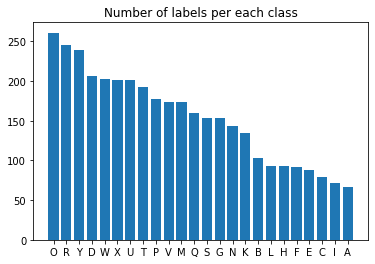
\includegraphics[width=\textwidth]{thesis/images/static_hand_gestures_dataset.png}
    \caption{Class distribution in the static hand gestures dataset.}
    \label{fig:class_distribution_static_hand_gestures}
\end{figure}

\subsubsection{Tests}
In table~\ref{tab:tests_static_hand_gestures}  the tests performed to find the best configuration to recognize static hand gestures are listed. ``Not defined'' in the column of ``Number of elements per class'' means that the whole dataset, described in~\ref{ss:dataset_static_gestures}, has been used to train the network.
\begin{table}[H]
\begin{tabular}{|c|c|c|}
\hline
\textbf{Test name}          & \textbf{Number of elements per class} & \textbf{Dropout rate} \\ \hline
full\_dataset               & Not defined                           & 0.0                   \\ \hline
full\_dataset\_dropout & Not defined                           & 0.2                   \\ \hline
10\_samples                 & 10                                    & 0.0                   \\ \hline
7\_samples                  & 7                                     & 0.0                   \\ \hline
6\_samples                  & 6                                     & 0.0                   \\ \hline
5\_samples                  & 5                                     & 0.0                   \\ \hline
\end{tabular}
\caption{Training configurations for the static hand gesture classifier.}\label{tab:tests_static_hand_gestures}
\end{table}
I mainly focused on finding the minimum amount of samples in order to obtain a good accuracy and a short training time. 

\subsubsection{Results}
The data gathered during the training are shown in table~\ref{tab:result_static_hand_gestures} and has been plotted. The graphs are shown in figure~\ref{fig:results_graphs_static_hand_gestures} and~\ref{fig:performances_dynamic_hand_gestures}.
\begin{table}[H]
\resizebox{\textwidth}{!}{%
\begin{tabular}{|c|c|c|c|}
\hline
\textbf{Test name}          & \textbf{Evaluation accuracy} & \textbf{Evaluation loss} & \textbf{Training time} \\ \hline
full\_dataset               & 0.99                         & 0.03                     & 6s 587ms               \\ \hline
full\_dataset\_dropout & 0.99                         & 0.01                     & 38s 769ms              \\ \hline
10\_samples                 & 1                            & 0.02                     & 26s 883ms              \\ \hline
7\_samples                  & 1                            & 0.04                     & 15s 804ms              \\ \hline
6\_samples                  & 1                            & 0.009                    & 31s 839ms              \\ \hline
5\_samples                  & 0.27                         & 2.90                     & 4s 551ms               \\ \hline
\end{tabular}%
}
\caption{Results for training the static hand gesture recognizer.}
\label{tab:result_static_hand_gestures}
\end{table}

\begin{figure}[H]
     \centering
     \begin{subfigure}[b]{0.45\textwidth}
         \centering
         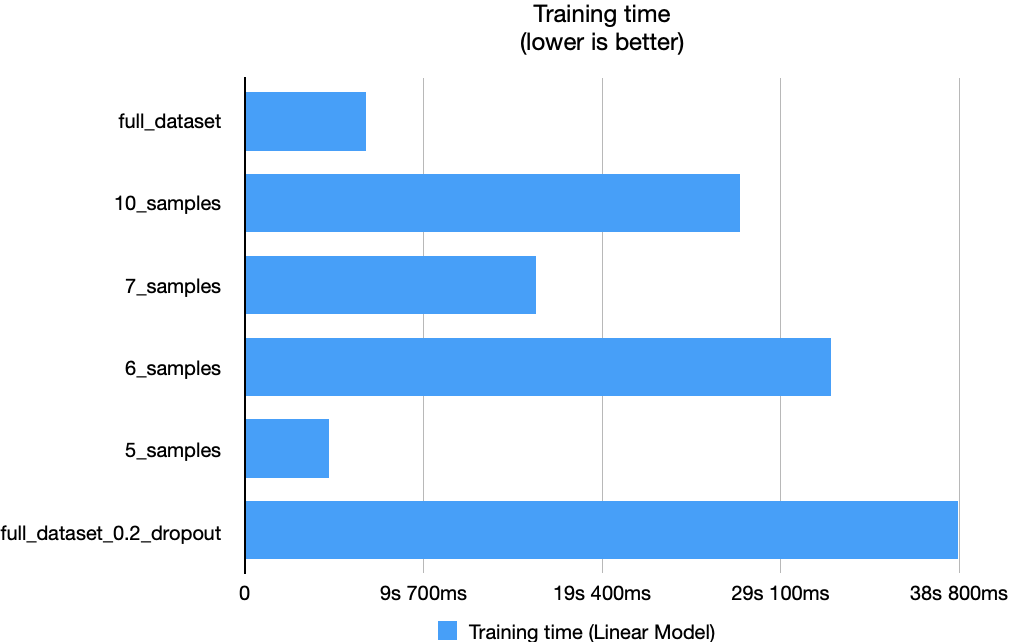
\includegraphics[width=\textwidth]{thesis/images/training_time_hand_gestures.png}
         \caption{Training time in tests static hand gestures.}
         \label{fig:training_time_static_hand_gestures}
     \end{subfigure}
     \hfill
     \begin{subfigure}[b]{0.45\textwidth}
         \centering
         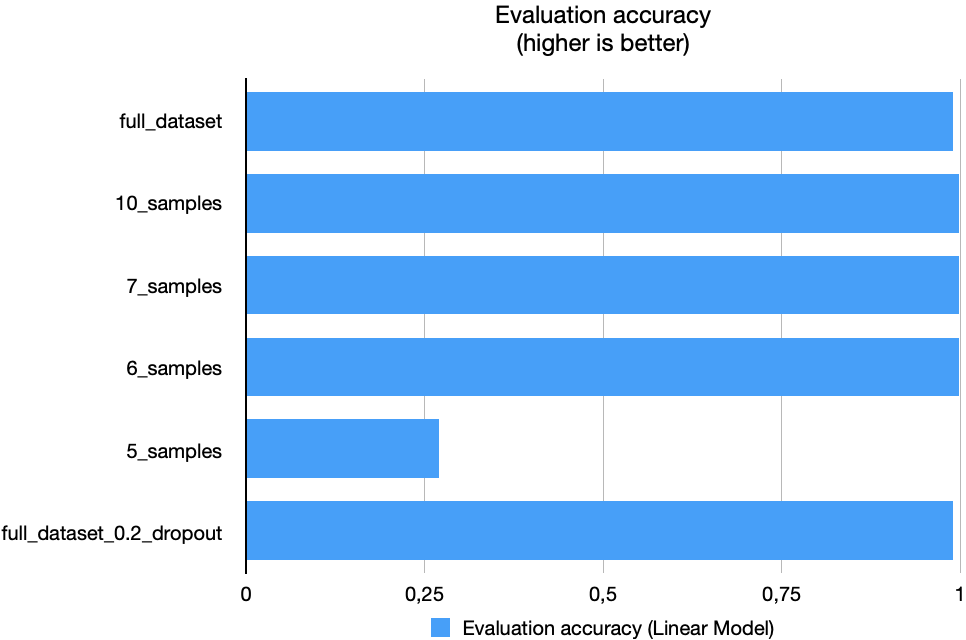
\includegraphics[width=\textwidth]{thesis/images/evaluation_accuracy_static_hand_gestures.png}
         \caption{Accuracy in tests static hand gestures.}
         \label{fig:evaluation_accuracy_static_hand_gestures}
     \end{subfigure}
     \hfill
     \begin{subfigure}[b]{0.45\textwidth}
         \centering
         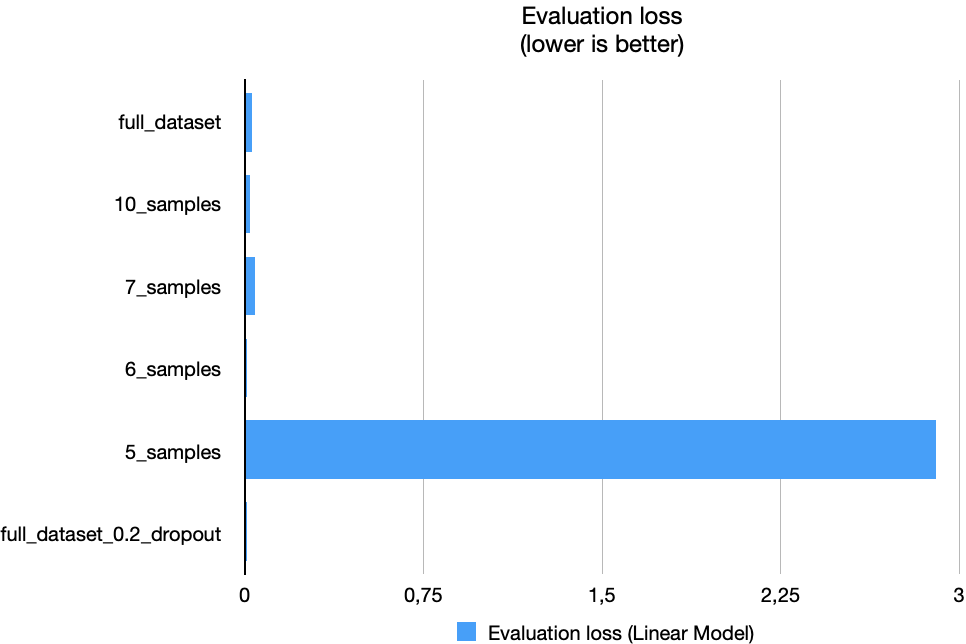
\includegraphics[width=\textwidth]{thesis/images/evaluation_loss_static_hand_gestures.png}
         \caption{Loss in tests static hand gestures.}
         \label{fig:evaluation_loss_static_hand_gestures.}
     \end{subfigure}
        \caption{Results graphs for the training of the static hand gesture recognizer}
        \label{fig:results_graphs_static_hand_gestures}
\end{figure}

\begin{figure}[H]
    \centering
    \begin{subfigure}[b]{\textwidth}
        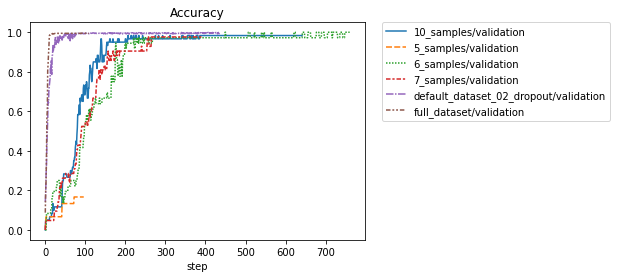
\includegraphics[width=\textwidth]{thesis/images/keypoint_accuracy.png}
        \caption{Accuracy performance in the different runs of the static hand gestures.}
        \label{fig:accuracy_performance_static_hand_gestures}
    \end{subfigure}
    \hfill
    \begin{subfigure}[b]{\textwidth}
        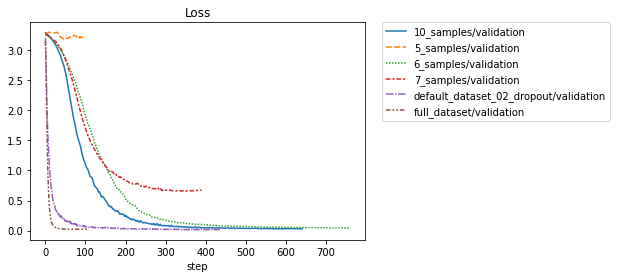
\includegraphics[width=\textwidth]{thesis/images/keypoint_loss.png}
        \caption{Loss performance in the different runs of the static hand gestures.}
        \label{fig:loss_performance_static_hand_gestures}
    \end{subfigure}
    \caption{Performances in the different runs of the static hand gestures.}
\end{figure}

\subsection{Dynamic hand gesture}

\subsubsection{Dataset}
Two datasets have been used:
\begin{itemize}
    \item \textbf{five\_fingers}: in this dataset the history of the tip of every finger has been saved. There are $461$ elements with a total size of $1.1MB$. Its class distribution is shown in figure~\ref{fig:class_distribution_dynamic_hand_gestures_five_fingers};
    \item \textbf{one\_finger}: in this dataset only the history of the tip of the index finger has been saved. There are $994$ elements with a total size of $423KB$. Its class distribution is shown in figure~\ref{fig:class_distribution_dynamic_hand_gestures_one_finger}.
\end{itemize}

\begin{figure}[H]
    \centering
    \begin{subfigure}[b]{0.45\textwidth}
        \centering
        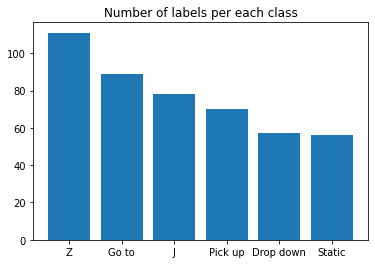
\includegraphics[width=\textwidth]{thesis/images/dynamic_hand_gestures_five_fingers.png}
        \caption{Class distribution in the dynamic hand gestures dataset with five fingers.}
        \label{fig:class_distribution_dynamic_hand_gestures_five_fingers}
    \end{subfigure}
    \hfill
    \begin{subfigure}[b]{0.45\textwidth}
        \centering
        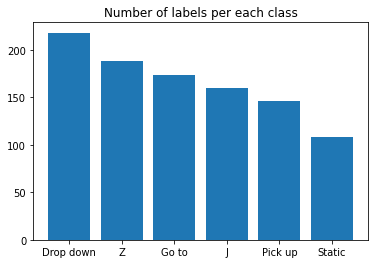
\includegraphics[width=\textwidth]{thesis/images/dynamic_hand_gestures_one_finger.png}
        \caption{Class distribution in the dynamic hand gestures dataset with one finger.}
        \label{fig:class_distribution_dynamic_hand_gestures_one_finger}
    \end{subfigure}
    \caption{Class distribution in the dynamic hand gestures datasets.}
    \label{fig:my_label}
\end{figure}

\subsubsection{Tests}
In table~\ref{tab:tests_dynamic_hand_gestures} the tests performed to find the best configuration to recognize dynamic hand gestures are listed. ``Not defined'' in the column ``Number of elements per class'' means that the whole dataset (specified in column ``Dataset'') has been used.
\begin{table}[H]
\resizebox{\textwidth}{!}{%
\begin{tabular}{|c|c|c|c|}
\hline
\textbf{Test name} & \textbf{Dataset} & \textbf{Network type} & \textbf{Number of elements per class} \\ \hline
full\_dataset      & five\_fingers    & feed\_forward         & Not defined                           \\ \hline
50\_samples        & five\_fingers    & feed\_forward         & 50                                    \\ \hline
10\_samples        & five\_fingers    & feed\_forward         & 10                                    \\ \hline
full\_dataset      & five\_fingers    & lstm                  & Not defined                           \\ \hline
50\_samples        & five\_fingers    & lstm                  & 50                                    \\ \hline
10\_samples        & five\_fingers    & lstm                  & 10                                    \\ \hline
full\_dataset      & one\_finger      & feed\_forward         & Not defined                           \\ \hline
50\_samples        & one\_finger      & feed\_forward         & 50                                    \\ \hline
10\_samples        & one\_finger      & feed\_forward         & 10                                    \\ \hline
\end{tabular}%
}
\caption{Training configurations for the dynamic hand gesture classifier.}
\label{tab:tests_dynamic_hand_gestures}
\end{table}

As for the static hand gesture recognizer, I focused on finding the minimum size of the dataset in order to obtain a good accuracy and a short training time.

\subsubsection{Results}
The data gathered during the training are shown in table~\ref{tab:result_dynamic_hand_gestures} and has been plotted. The graphs are shown in figure~\ref{fig:results_graphs_dynamic_hand_gestures} and~\ref{fig:performances_dynamic_hand_gestures}.
\begin{table}[H]
\resizebox{\textwidth}{!}{%
\begin{tabular}{|c|c|c|c|c|c|}
\hline
\textbf{Test name} & \textbf{Dataset} & \textbf{Network type} & \textbf{Evaluation accuracy} & \textbf{Evaluation loss} & \textbf{Training time} \\ \hline
full\_dataset      & five\_fingers    & feed\_forward         & 0.98                         & 0.02                     & 19s 878ms              \\ \hline
50\_samples        & five\_fingers    & feed\_forward         & 0.97                         & 0.04                     & 14s 558ms              \\ \hline
10\_samples        & five\_fingers    & feed\_forward         & 0.77                         & 1,27                     & 16s 970ms              \\ \hline
full\_dataset      & five\_fingers    & lstm                  & 0.98                         & 0.01                     & 22s 110ms              \\ \hline
50\_samples        & five\_fingers    & lstm                  & 0.97                         & 0.03                     & 24s 161ms              \\ \hline
10\_samples        & five\_fingers    & lstm                  & 0.66                         & 0.95                     & 14s 798ms              \\ \hline
full\_dataset      & one\_finger      & feed\_forward         & 0.93                         & 0.21                     & 38s 749ms              \\ \hline
50\_samples        & one\_finger      & feed\_forward         & 0.95                         & 0.26                     & 42s 535ms              \\ \hline
10\_samples        & one\_finger      & feed\_forward         & 0                            & 1.82                     & 2s 622ms               \\ \hline
\end{tabular}%
}
\caption{Results for training the dynamic hand gesture recognizer.}
\label{tab:result_dynamic_hand_gestures}
\end{table}

\begin{figure}[H]
     \centering
     \begin{subfigure}[b]{0.45\textwidth}
         \centering
         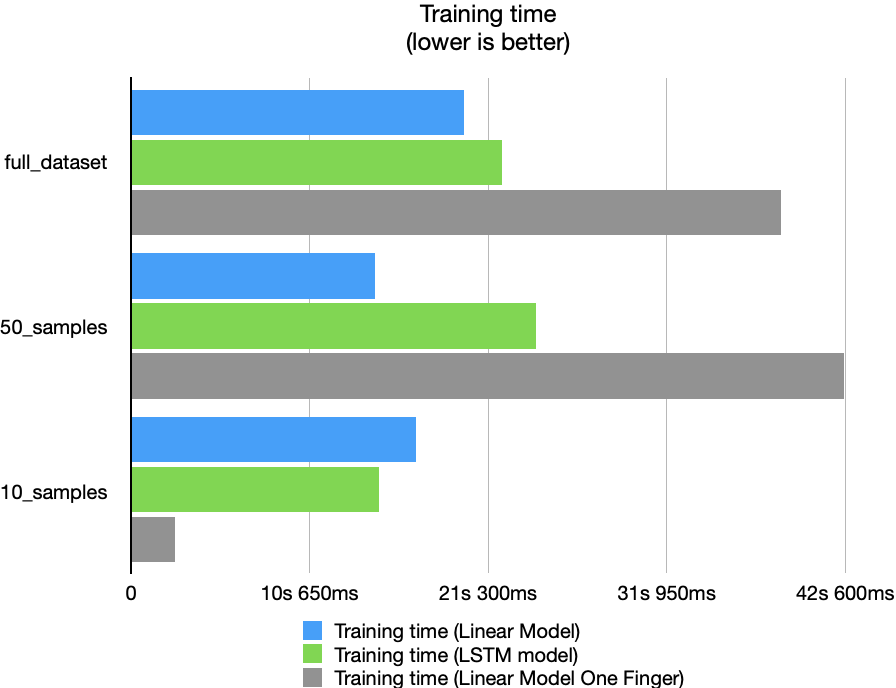
\includegraphics[width=\textwidth]{thesis/images/training_time_dynamic_hand_gestures.png}
         \caption{Training time in tests dynamic hand gestures.}
         \label{fig:training_time_dynamic_hand_gestures}
     \end{subfigure}
     \hfill
     \begin{subfigure}[b]{0.45\textwidth}
         \centering
         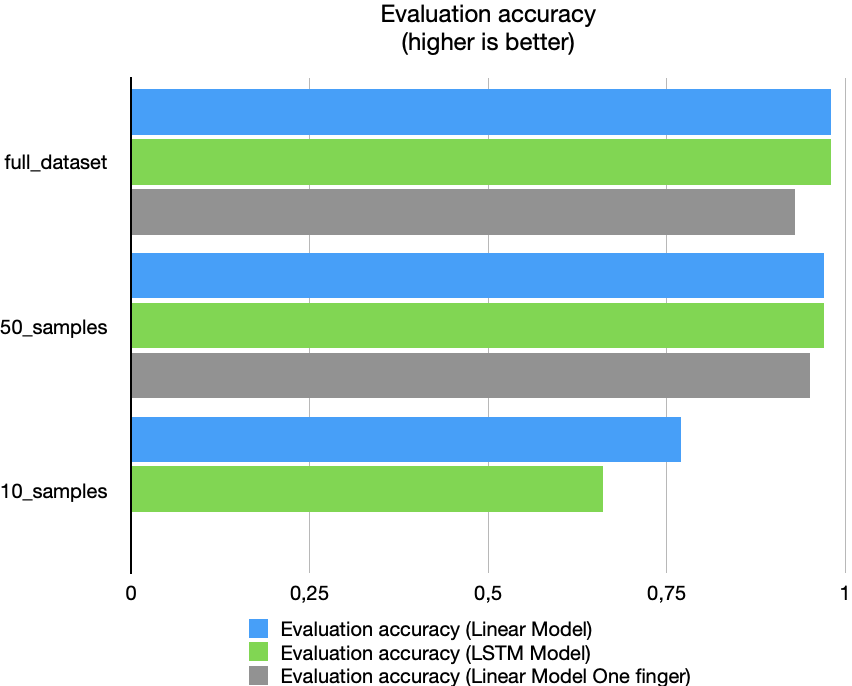
\includegraphics[width=\textwidth]{thesis/images/evaluation_accuracy_dynamic_hand_gestures.png}
         \caption{Accuracy in tests dynamic hand gestures.}
         \label{fig:evaluation_accuracy_dynamic_hand_gestures}
     \end{subfigure}
     \hfill
     \begin{subfigure}[b]{0.45\textwidth}
         \centering
         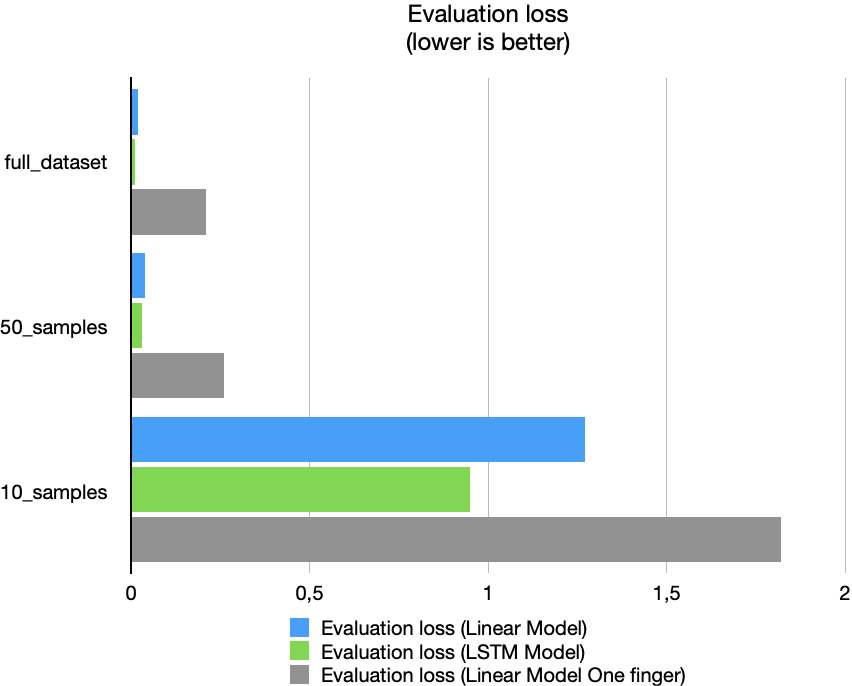
\includegraphics[width=\textwidth]{thesis/images/evaluation_loss_dynamic_hand_gestures.png}
         \caption{Loss in tests dynamic hand gestures.}
         \label{fig:evaluation_loss_dynamic_hand_gestures.}
     \end{subfigure}
        \caption{Results graphs for the training of the dynamic hand gesture recognizer}
        \label{fig:results_graphs_dynamic_hand_gestures}
\end{figure}

\begin{figure}[H]
\centering
\begin{subfigure}[b]{\textwidth}
    \centering
    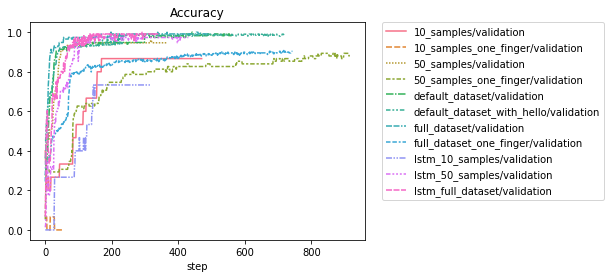
\includegraphics[width=\textwidth]{thesis/images/point_history_accuracy.png}
    \caption{Accuracy performance in the different runs of the dynamic hand gestures.}
    \label{fig:accuracy_performance_dynamic_hand_gestures}
\end{subfigure}
\hfill
\begin{subfigure}[b]{\textwidth}
    \centering
    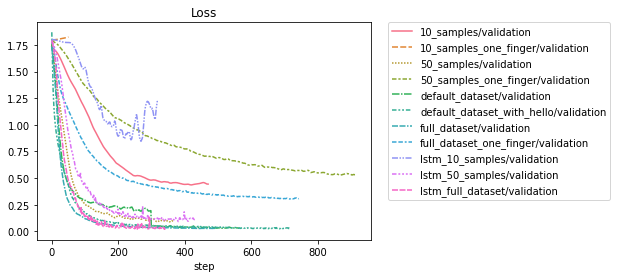
\includegraphics[width=\textwidth]{thesis/images/point_history_loss.png}
    \caption{Loss performance in the different runs of the dynamic hand gestures.}
    \label{fig:loss_performance_dynamic_hand_gestures}
\end{subfigure}
\caption{Performances in the different runs of the dynamic hand gestures.}
\label{fig:performances_dynamic_hand_gestures}
\end{figure}

\subsection{System resource usage during training}\label{ss:system_resource_usage_training}
A test has been performed to collect data on the use of system resources, in particular CPU and RAM usage. I added one new static and one new dynamic gesture and then I used the method described in section~\ref{ss:system_resource_utilization} to collect the usage of CPU and RAM of the program during the training process. The training process has been executed on the host machine and not in the virtual machine. The figures~\ref{fig:system_resource_graphs_static_training} and~\ref{fig:system_resource_graphs_dynamic_training} show the results obtained.

\begin{figure}[H]
    \centering
    \begin{subfigure}[b]{0.45\textwidth}
        \centering
        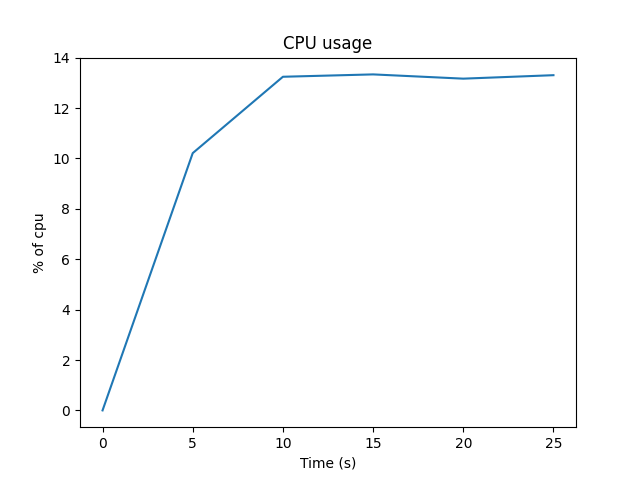
\includegraphics[width=\textwidth]{thesis/images/cpu_static_training.png}
        \caption{CPU usage.}
        \label{fig:cpu_usage_static_training}
    \end{subfigure}
    \hfill
    \begin{subfigure}[b]{0.45\textwidth}
        \centering
        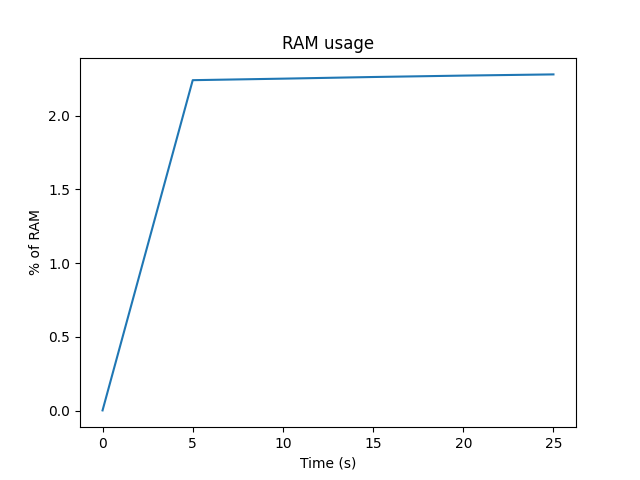
\includegraphics[width=\textwidth]{thesis/images/ram_static_training.png}
        \caption{RAM usage.}
        \label{fig:ram_usage_static_training}
    \end{subfigure}
    \caption{System resource utilization during the static gesture recognizer training}
    \label{fig:system_resource_graphs_static_training}
\end{figure}

\begin{figure}[H]
    \centering
    \begin{subfigure}[b]{0.45\textwidth}
        \centering
        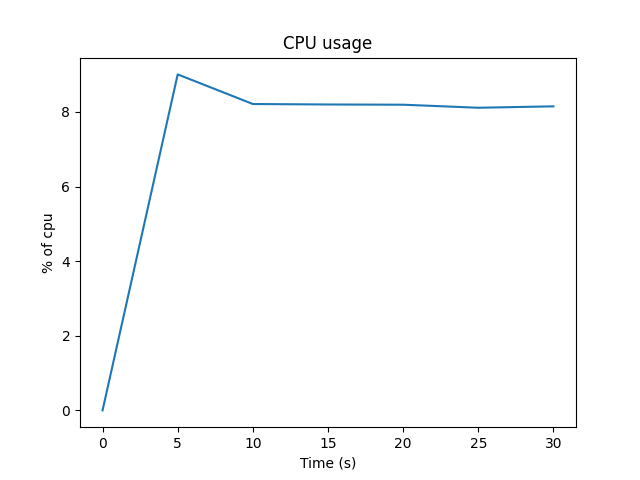
\includegraphics[width=\textwidth]{thesis/images/cpu_dynamic_training.png}
        \caption{CPU usage.}
        \label{fig:cpu_usage_dynamic_training}
    \end{subfigure}
    \hfill
    \begin{subfigure}[b]{0.45\textwidth}
        \centering
        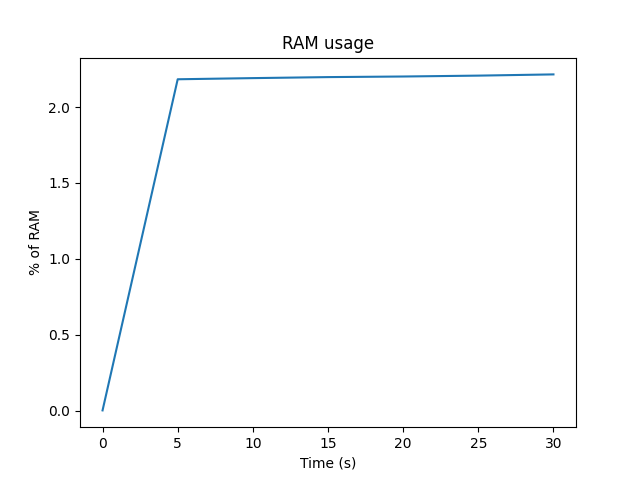
\includegraphics[width=\textwidth]{thesis/images/ram_dynamic_training.png}
        \caption{RAM usage.}
        \label{fig:ram_usage_dynamic_training}
    \end{subfigure}
    \caption{System resource utilization during the dynamic gesture recognizer training}
    \label{fig:system_resource_graphs_dynamic_training}
\end{figure}

\section{Integration with ROS}
Three incremental tests have been performed to test the correct integration with \gls{ROS}:
\begin{enumerate}
    \item message exchange: the first test was about the exchange of different messages when different gestures were recognized;
    \item navigation system: the next step was the correct integration with the navigation system ``Nav2'' in a simple environment;
    \item complex scenario: the last test carried on was on a more real scenario, a robot in a warehouse doing different tasks.
\end{enumerate}

In these three tests the network topology was similar:
\begin{itemize}
    \item the framework creates a node to communicate with the rest of the network;
    \item the simulated robot could be considerated like another node;
    \item when the navigation system was integrated, it could be considered like another node.
\end{itemize}

The framework's node communicates with the other two nodes and, obviously, the navigation system's node communicates with the robot to tell it where it has to go. Figure~\ref{fig:ros_network_topology} shows the network topology implemented to carry on the tests.

\begin{figure}[H]
    \centering
    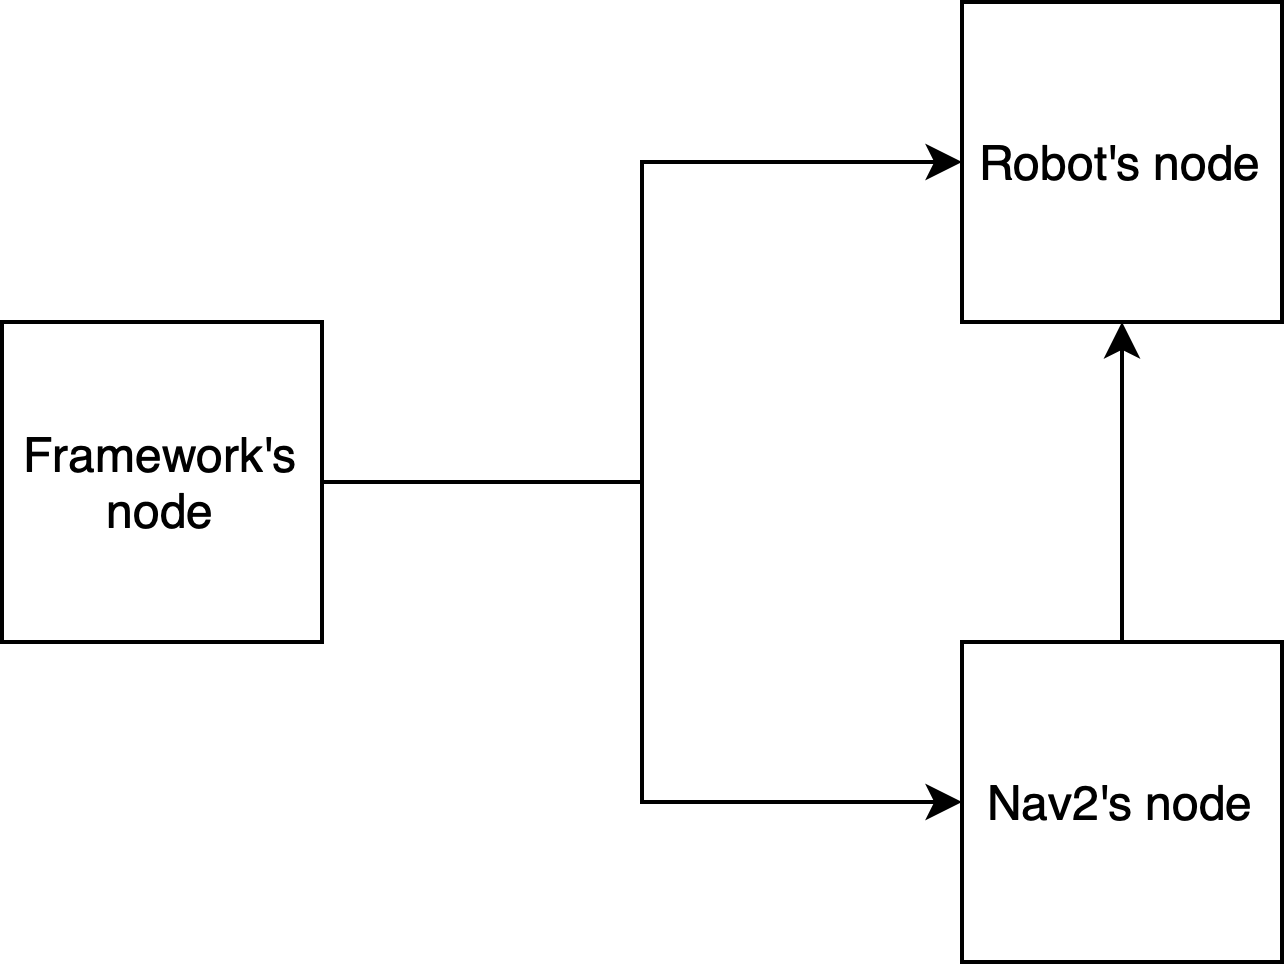
\includegraphics[width=0.6\textwidth]{thesis/images/ros_network_topology.png}
    \caption{ROS' network topology}
    \label{fig:ros_network_topology}
\end{figure}

\subsection{Integration with ROS' topic}
The first results achieved by integrating the framework with \gls{ROS} have been about the communication between two nodes: the one representing the hand gestures recognizer and the \textit{TurtleSim}. \textit{TurtleSim} is a ``simulator'' provided by \gls{ROS} which takes inspiration from the turtle programming languages, where you control a turtle by telling it to go forward, turn left, and turn right. The turtle has a pen attached to it that draws the path on the screen. Figure~\ref{fig:initial_turtlesim} shows what it looks like at the startup.

\begin{figure}[H]
    \centering
    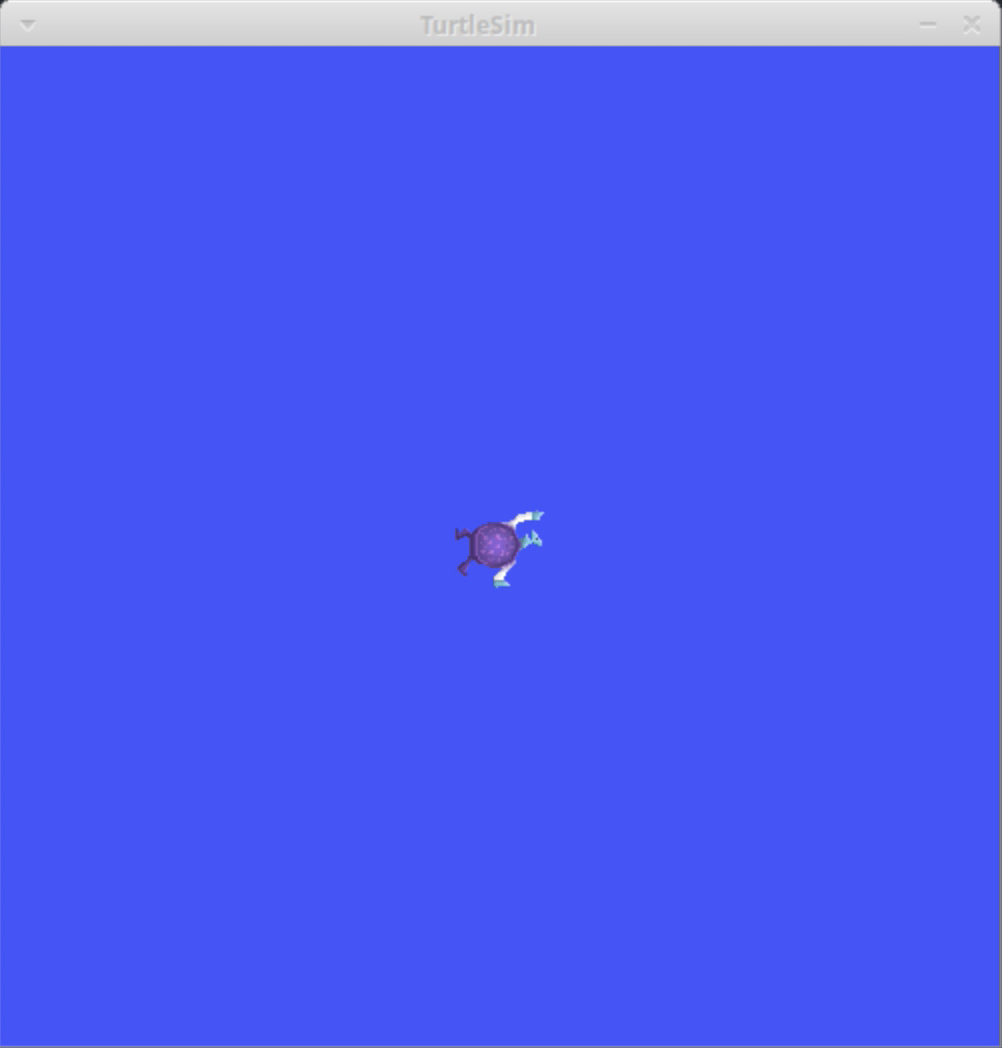
\includegraphics[width=0.4\textwidth]{thesis/images/initial_turtlesim.png}
    \caption{TurtleSim}
    \label{fig:initial_turtlesim}
\end{figure}

At this point in the implementation, the hand gesture recognizer creates a node and communicates with the \textit{TurtleSim} exchanging messages on two topics. The messages sent represented the direction and the velocity of the turtle. Four positions were defined, each of them linked to a static hand gesture (A, B, C, and D). Based on the gesture recognized, a sequence of messages were picked and sent to the turtle. These messages told the turtle how to reach the target position from its current position.

\begin{figure}[H]
     \centering
     \begin{subfigure}[b]{0.45\textwidth}
         \centering
         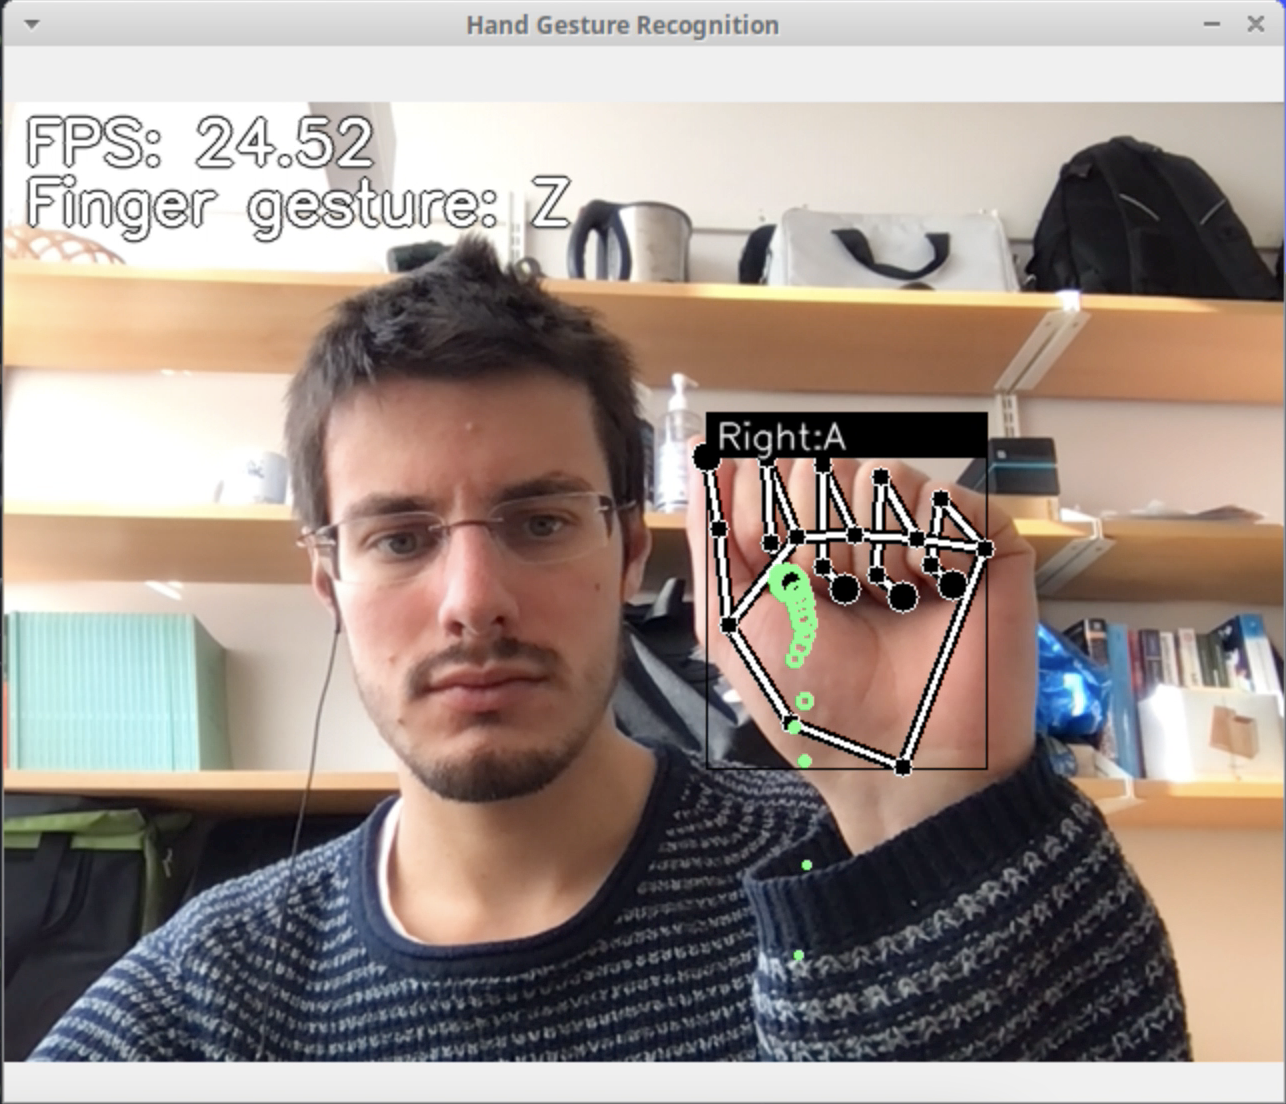
\includegraphics[width=\textwidth]{thesis/images/ARecognizedTurtleSim.png}
         \caption{Recognition of the `A' gesture.}
         \label{fig:A_gesture_recognition_turtlesim}
     \end{subfigure}
     \hfill
     \begin{subfigure}[b]{0.45\textwidth}
         \centering
         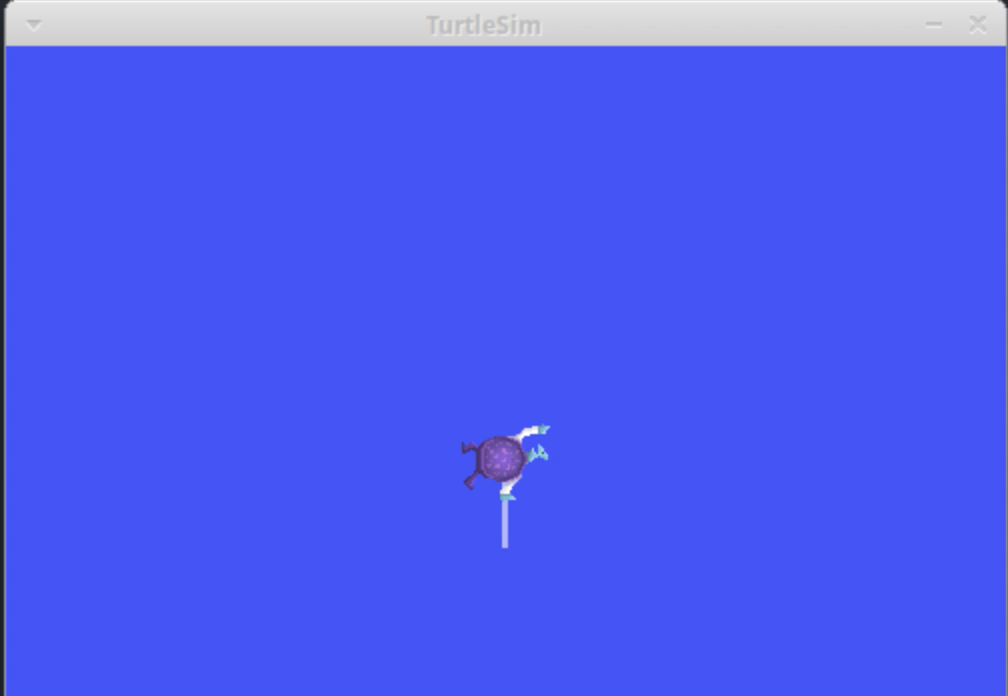
\includegraphics[width=\textwidth]{thesis/images/TurtleStartMoving.png}
         \caption{Turtle starts moving.}
         \label{fig:turtle_start_turtle_sim}
     \end{subfigure}
     \hfill
     \begin{subfigure}[b]{0.45\textwidth}
         \centering
         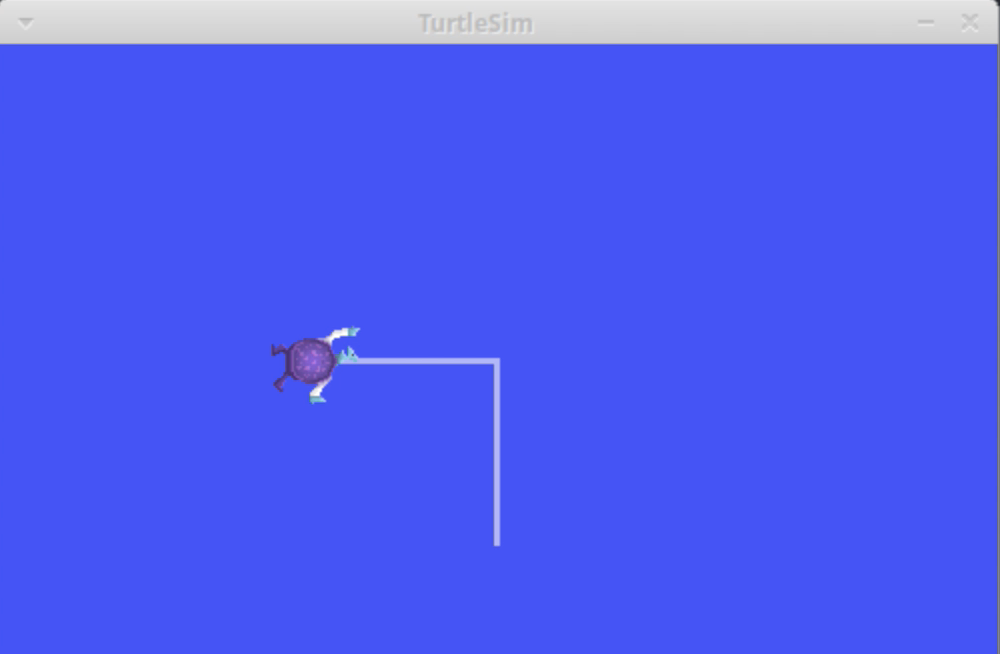
\includegraphics[width=\textwidth]{thesis/images/TurtleReachA.png}
         \caption{Turtle reaches position `A'.}
         \label{fig:turtle_reach_A_position.}
     \end{subfigure}
        \caption{Recognition of the `A' gesture and turtle movement toward position `A'.}
        \label{fig:example_to_A_turtlesim}
\end{figure}

\subsection{Integration with the navigation system}
The next step has been testing the integration with the navigation system ``Nav2''. I translated the test made with the \textit{TurtleSim} in a Gazebo World. The map used was an empty map (figure~\ref{fig:gazebo_empty_world}) to ensure that communication between the hand gesture recognizer and the navigation system is working properly. The test had been successful and the simulated robot moved into the correct position. Figure~\ref{fig:rviz_emptyworld} shows the RViz tool, which is integrated with the navigation system and shows the path the robot is following. RViz also gives some feedback and actions regarding the navigation status, as figure~\ref{fig:rviz_feedback} shows.

\begin{figure}[H]
    \centering
    \begin{subfigure}[b]{0.45\textwidth}
        \centering
        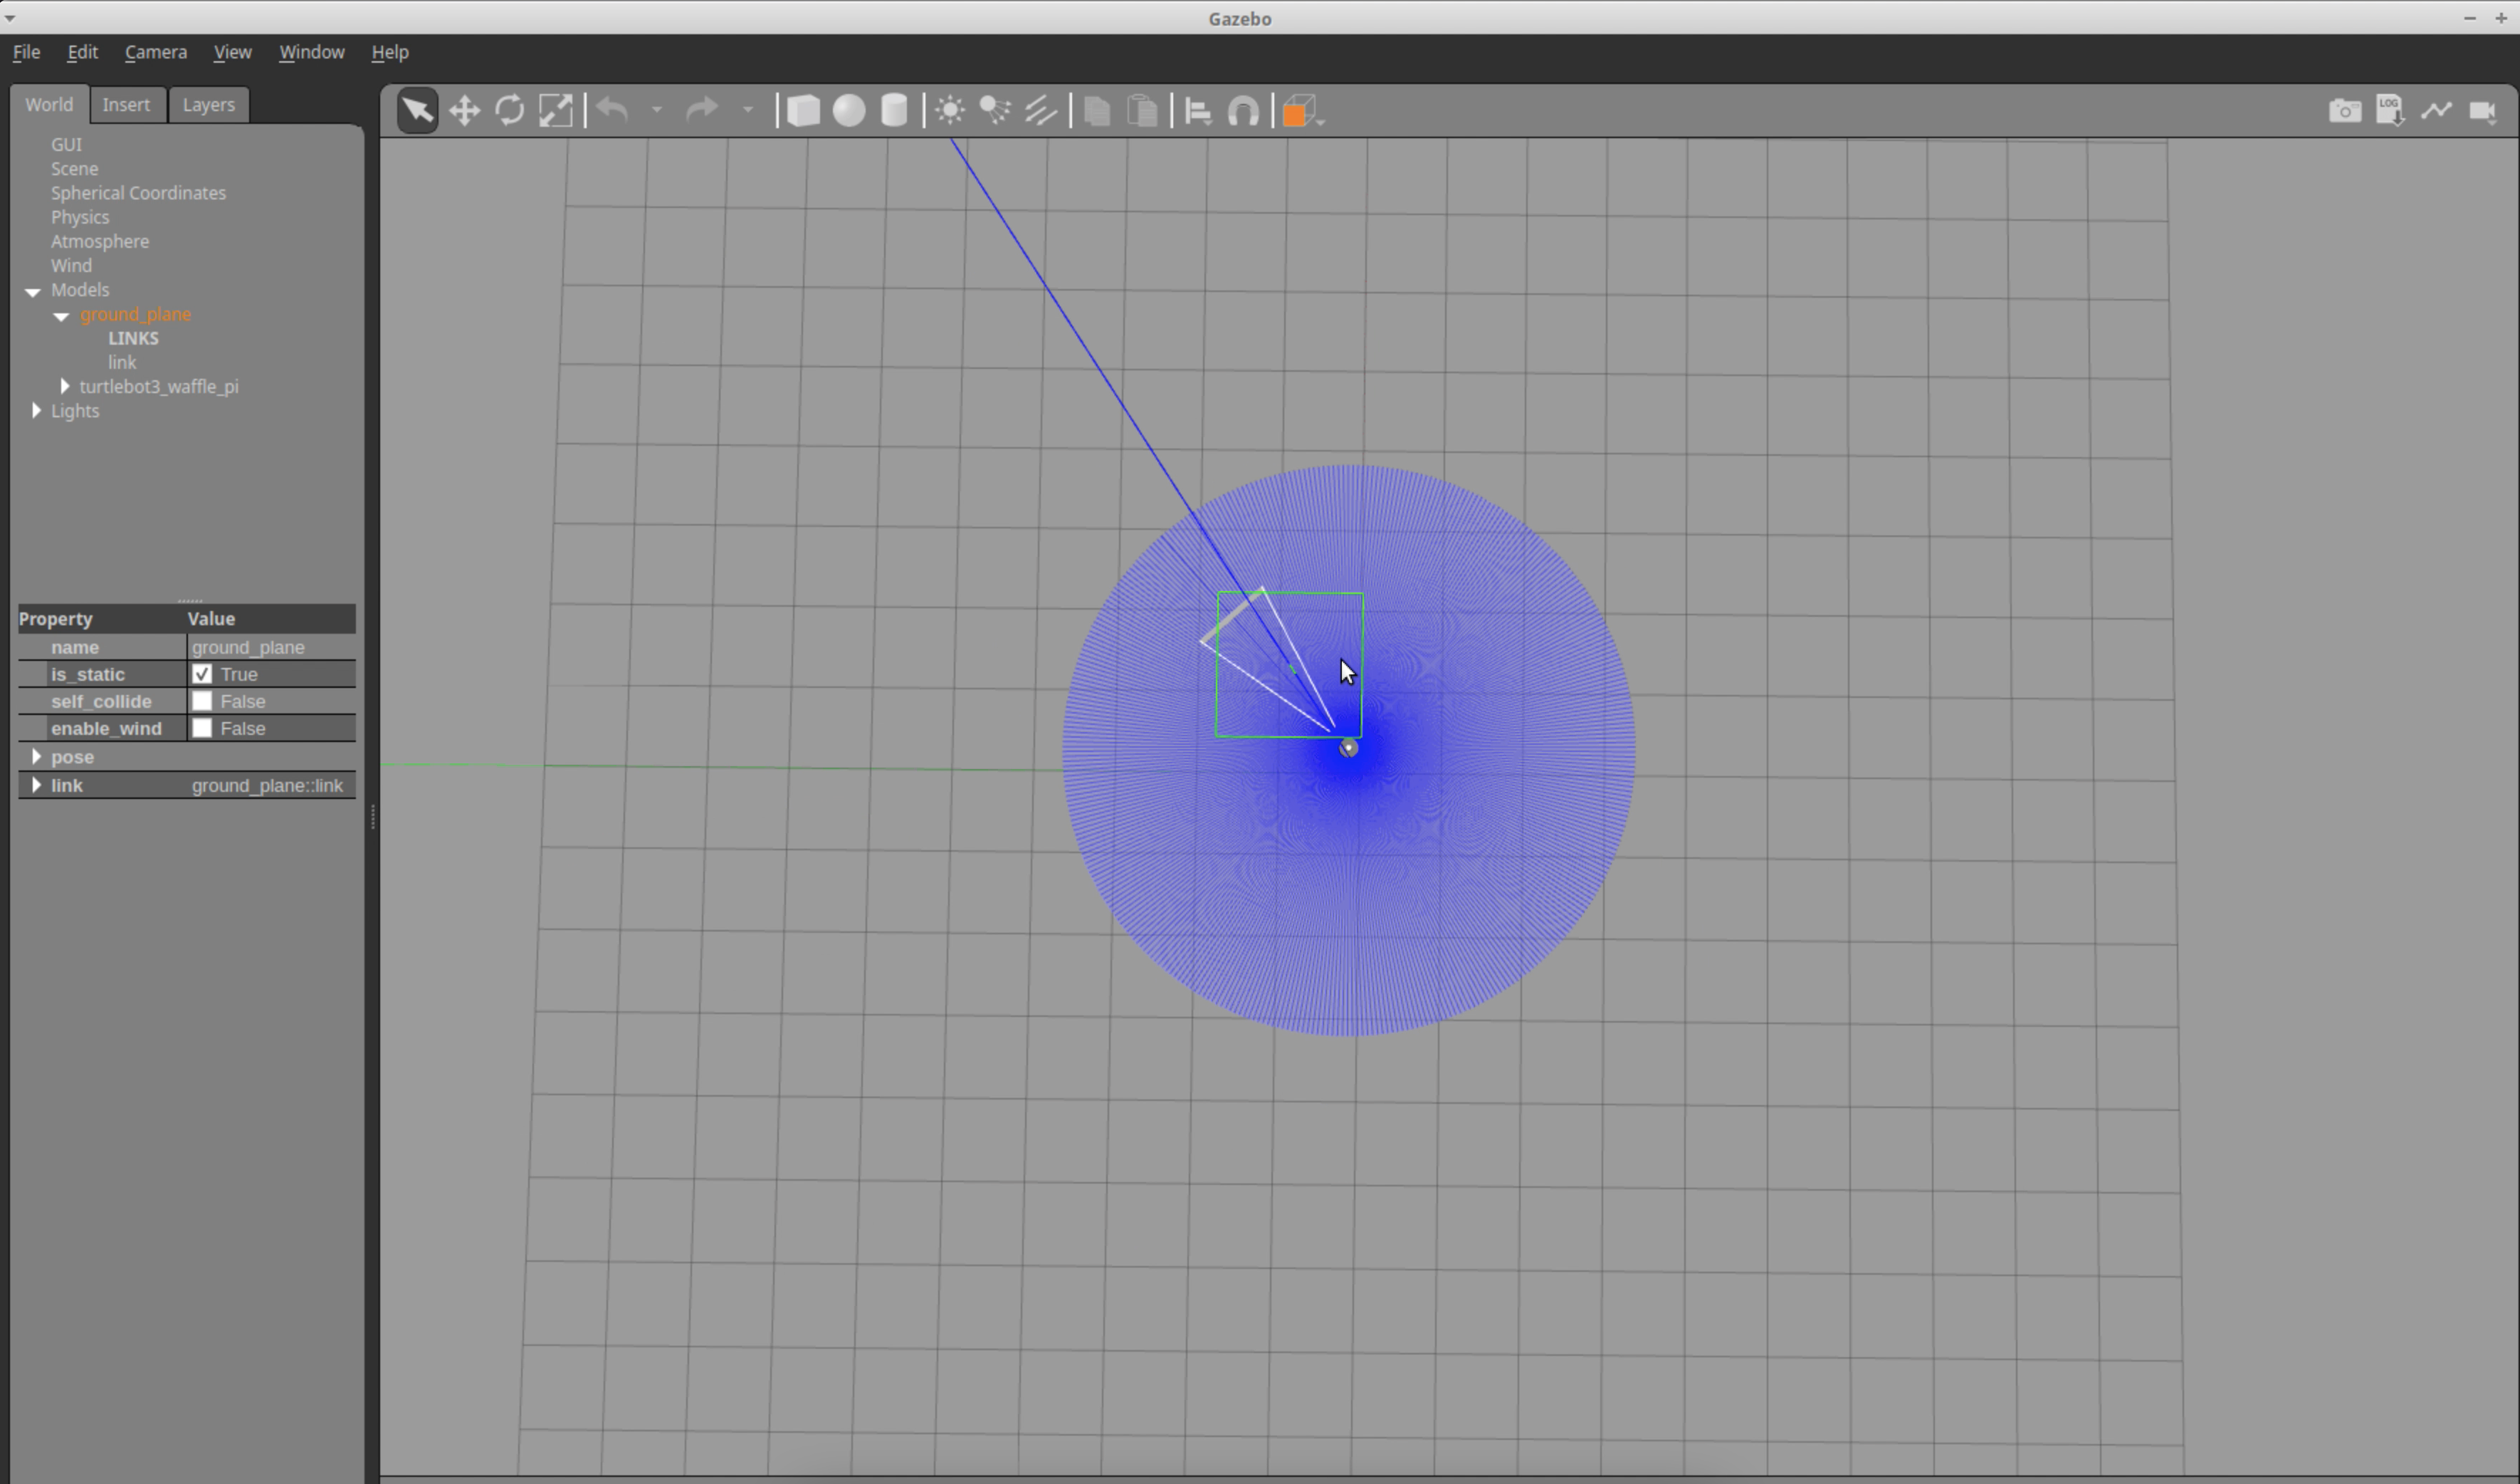
\includegraphics[width=\textwidth]{thesis/images/emptyGazeboWorld.png}
        \caption{Gazebo Empty World.}
        \label{fig:gazebo_empty_world}
    \end{subfigure}
    \hfill
    \begin{subfigure}[b]{0.45\textwidth}
        \centering
        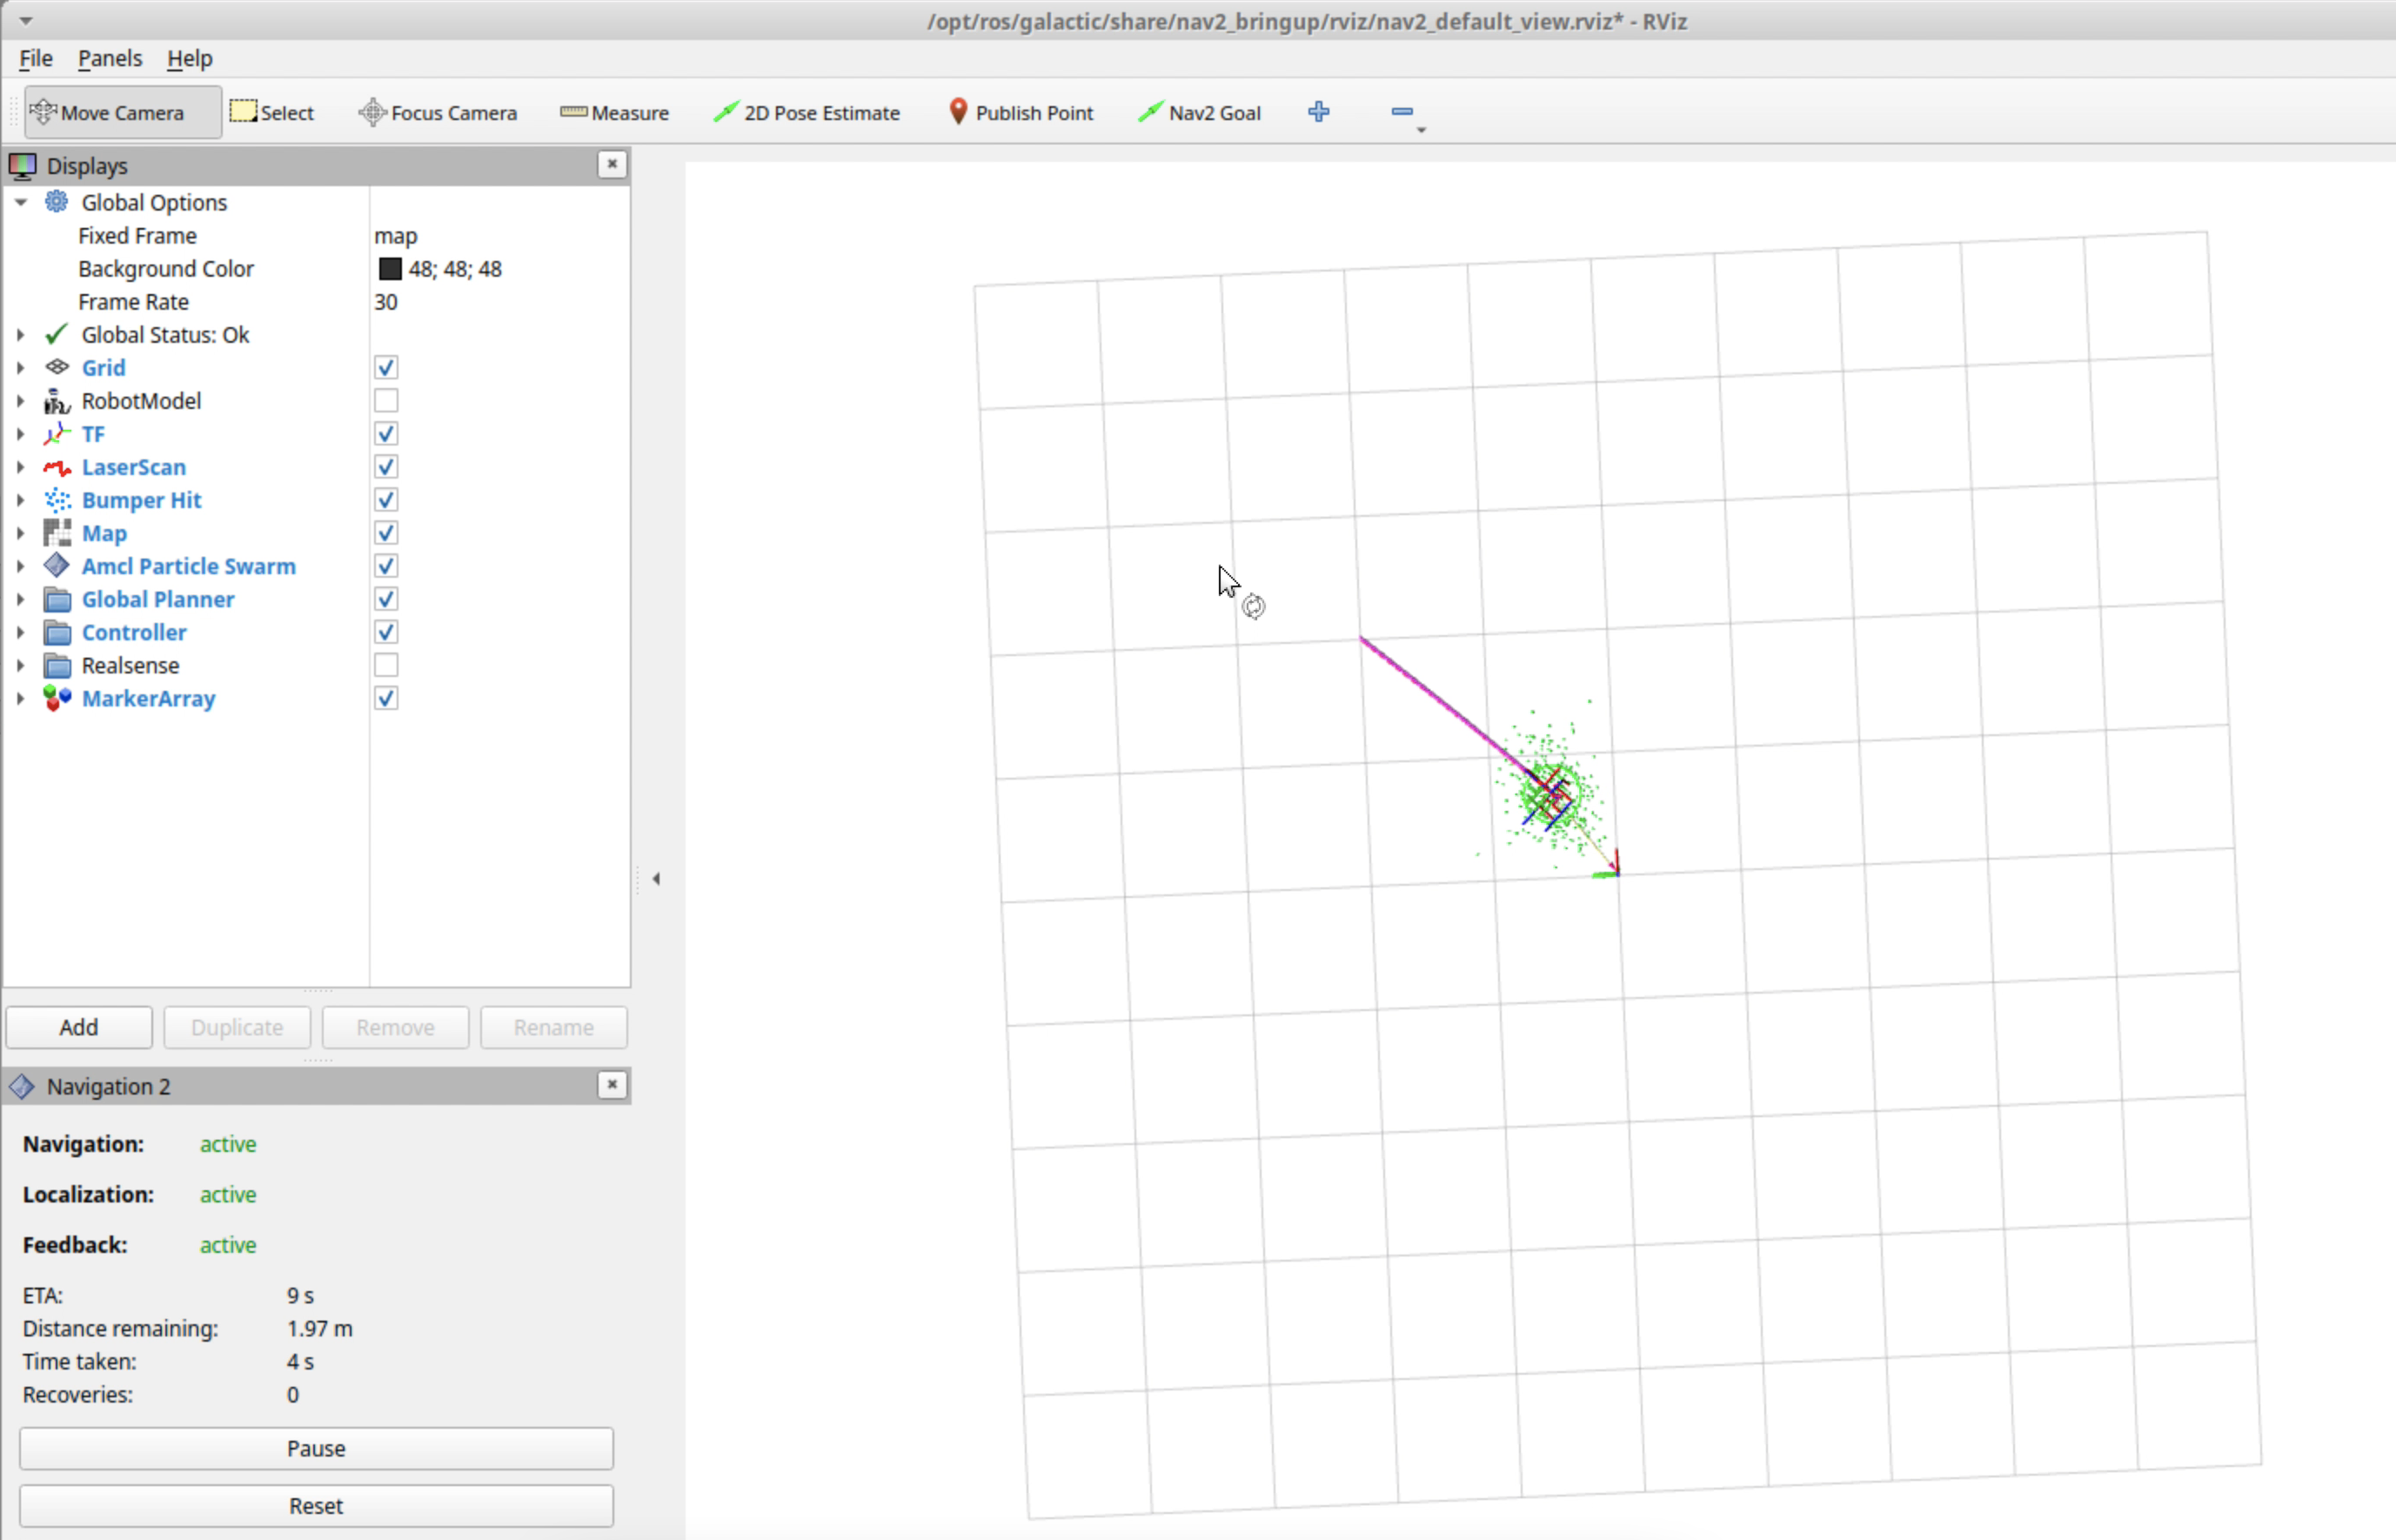
\includegraphics[width=\textwidth]{thesis/images/RVizPathEmptyWorld.png}
        \caption{RViz showing the path to position `A'.}
        \label{fig:rviz_emptyworld}
    \end{subfigure}
    \caption{Test navigation system in a Gazebo Empty World.}
    \label{fig:navigation_empty_gazebo_world}
\end{figure}

\begin{figure}[H]
    \centering
    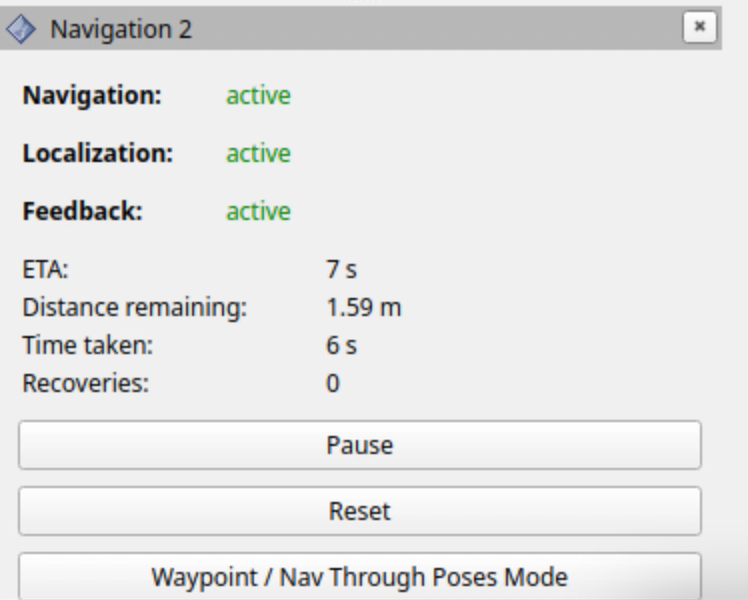
\includegraphics[width=0.4\textwidth]{thesis/images/feedbackRViz.png}
    \caption{RViz detail - feedback and actions.}
    \label{fig:rviz_feedback}
\end{figure}

\subsection{Test in a warehouse environment}

The last test to carry on regarding the integration with \gls{ROS} was in a more real scenario. The small warehouse environment provided by amazon\footnote{\href{https://github.com/aws-robotics/aws-robomaker-small-warehouse-world}{https://github.com/aws-robotics/aws-robomaker-small-warehouse-world}}, shown in figure~\ref{fig:small_warehouse_gazebo_world}, has been chosen to test the framework's final implementation with the automaton described in~\ref{ss:automaton_description}. In the world, the \textit{TurtleBot v3} has been inserted, which executes commands given via hand gestures recognized by the framework.

\begin{figure}[H]
    \centering
    \includegraphics[width=1\textwidth]{thesis/images/smallwarehouse.png}
    \caption{AWS Robomaker's small warehouse Gazebo world}
    \label{fig:small_warehouse_gazebo_world}
\end{figure}

When a complex world is used, RViz provides more interesting data. It displays the obstacles seen by the robot as well as the path computed by the ``Nav2'' algorithm to avoid them, for example. Figure~\ref{fig:rviz_smallwarehouse} shows the RViz's interface when the small warehouse world is loaded.

\begin{figure}[H]
    \centering
    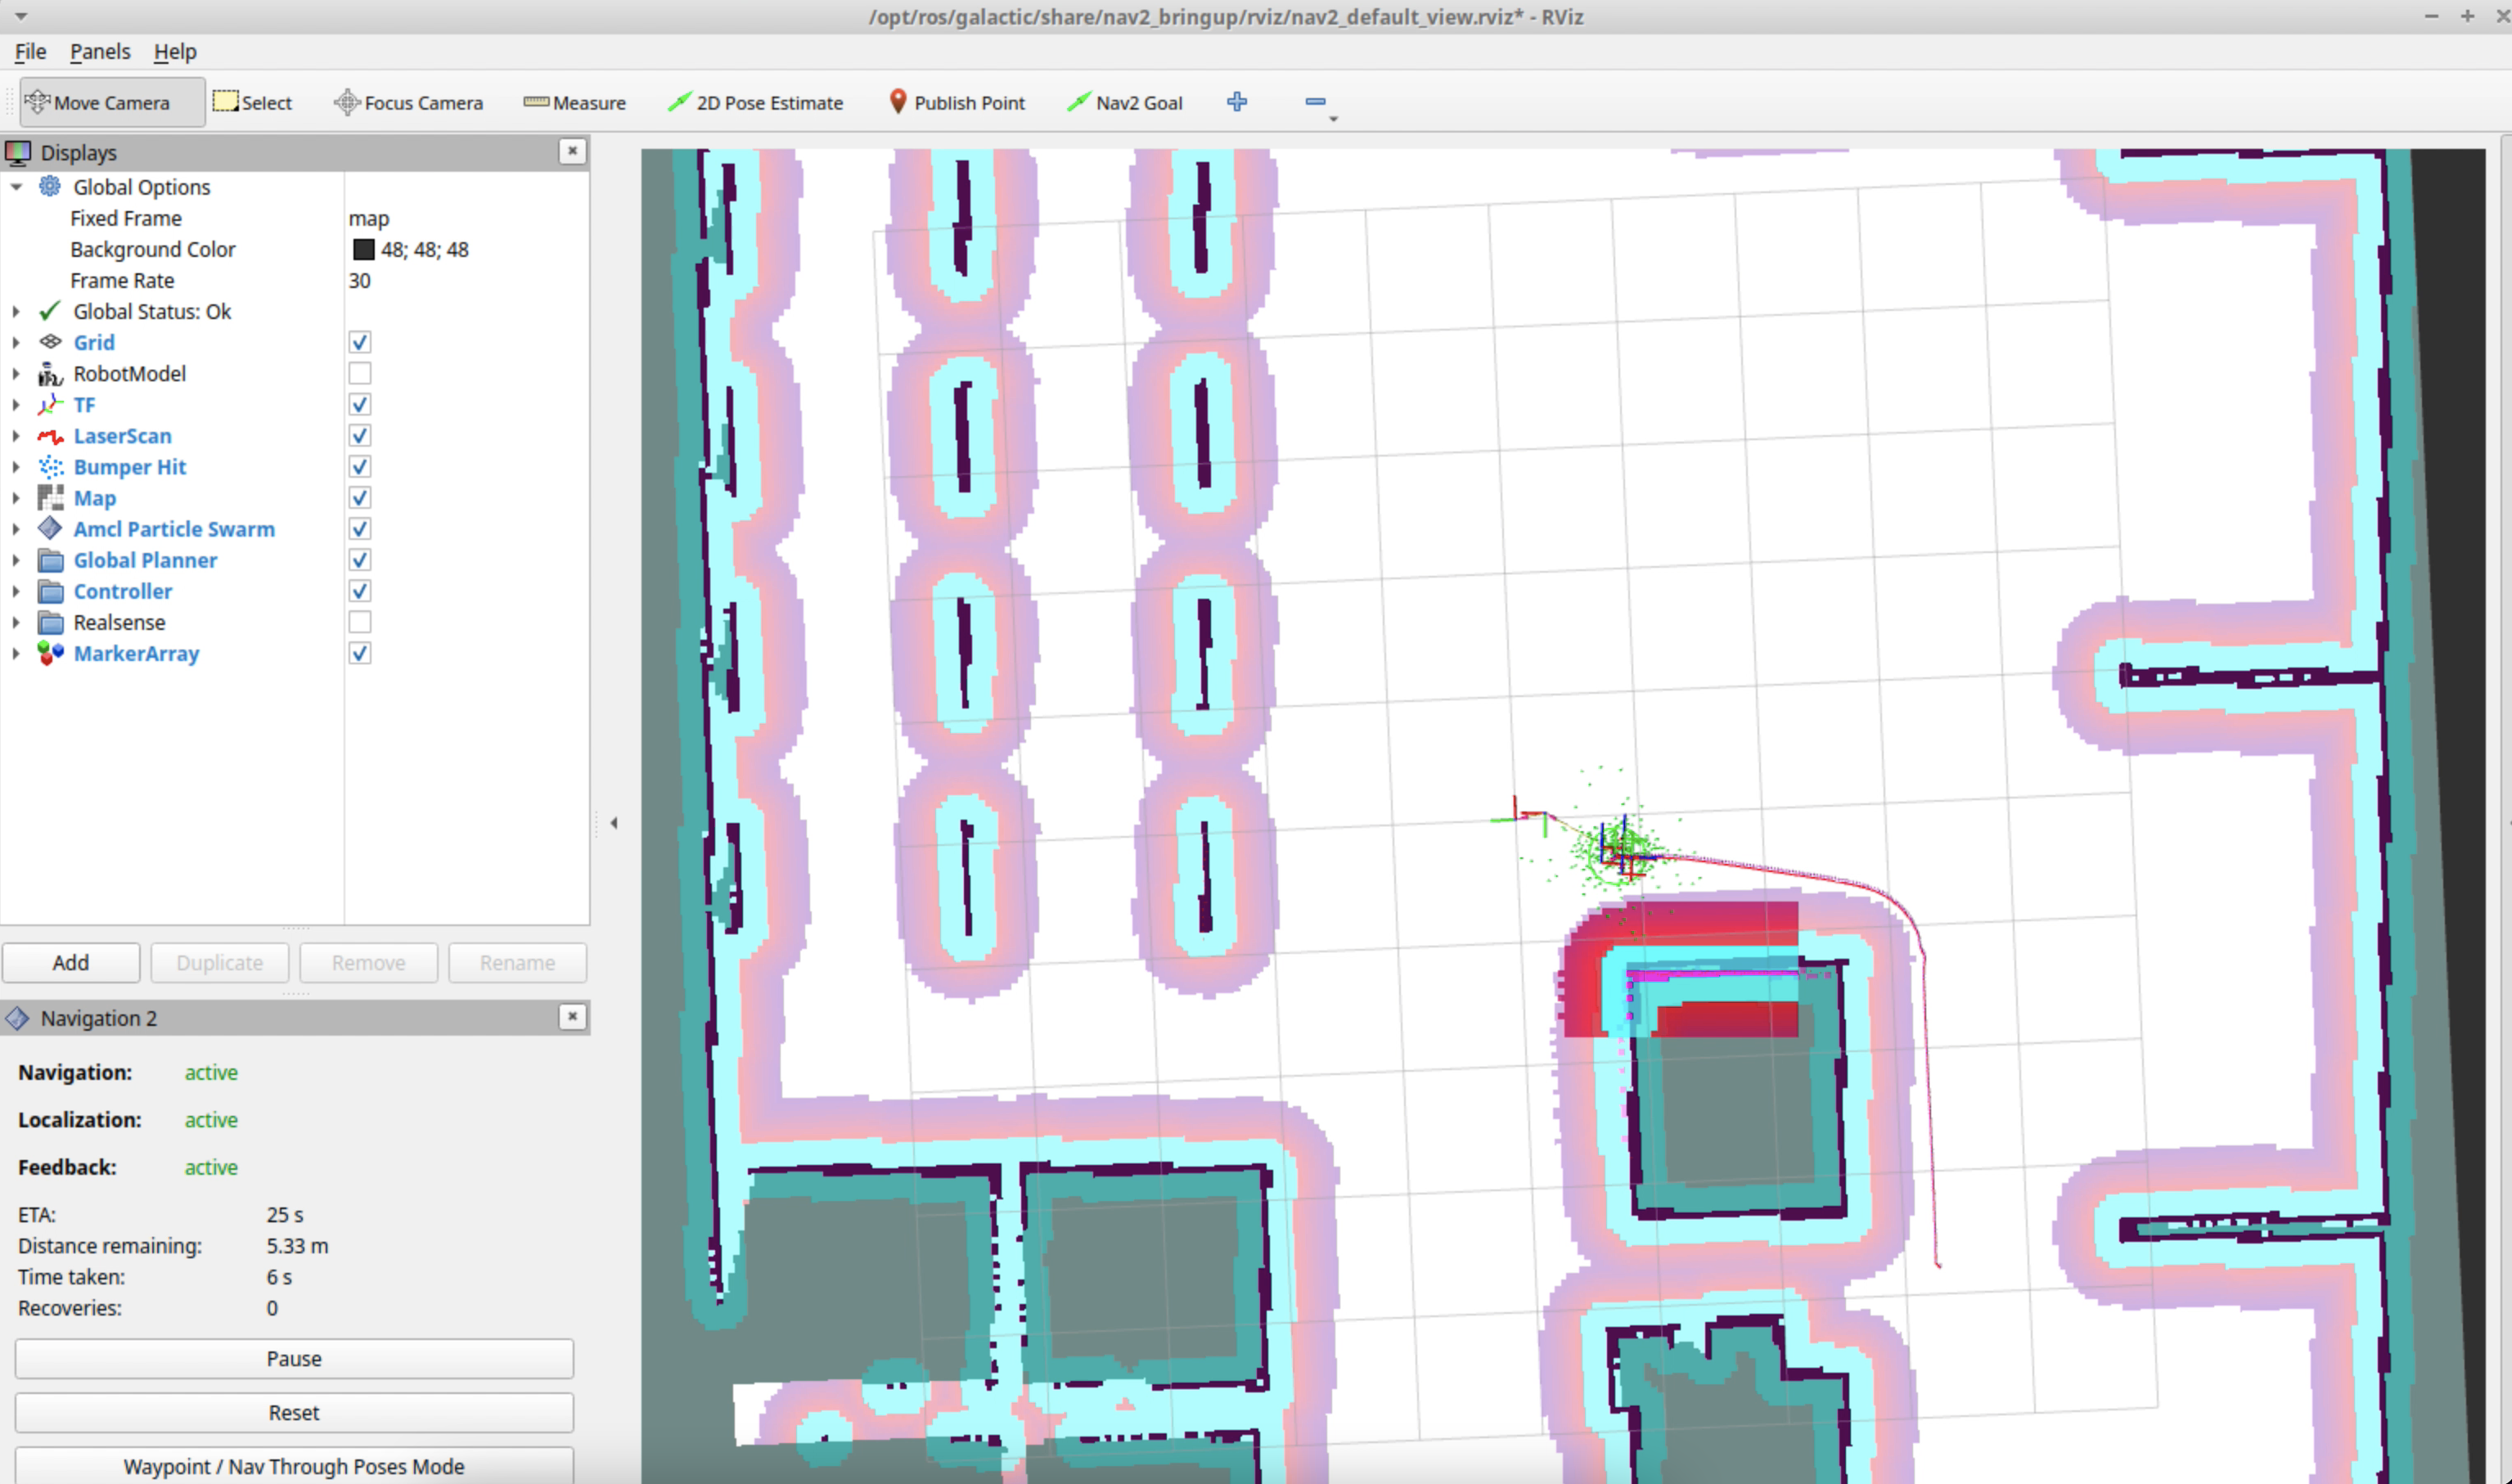
\includegraphics[width=1\textwidth]{thesis/images/rviz_smallwarehouse.png}
    \caption{RViz's interface during simulation in the small warehouse world.}
    \label{fig:rviz_smallwarehouse}
\end{figure}


The test carried on regarding the recognition of several sequences of gestures involving both dynamic and static hand gestures, the set of navigation goals, and the proper reception of some messages exchanged on a \gls{ROS}' topic. Moreover, with this whole environment set up, some data has been gathered during the simulation to prove the capabilities and lightness of the framework.

\subsection{System resource usage}
As in~\ref{ss:system_resource_usage_training}, a tests has been performed to gather some data about the system resource usage during the execution of the program in \texttt{operational mode}. This test has been executed in the virtual machine. I ran the simulator and the navigation tool. Then, I used the method described in section~\ref{ss:system_resource_utilization} to collect the usage of CPU and RAM of the program. I performed the following sequence of gesture:
\begin{enumerate}
    \item Go to;
    \item B;
    \item Pick up;
    \item D;
    \item Go to;
    \item C;
    \item Drop down.
\end{enumerate}
The results are shown in figure~\ref{fig:system_resource_graphs}

\begin{figure}[H]
    \centering
    \begin{subfigure}[b]{0.45\textwidth}
        \centering
        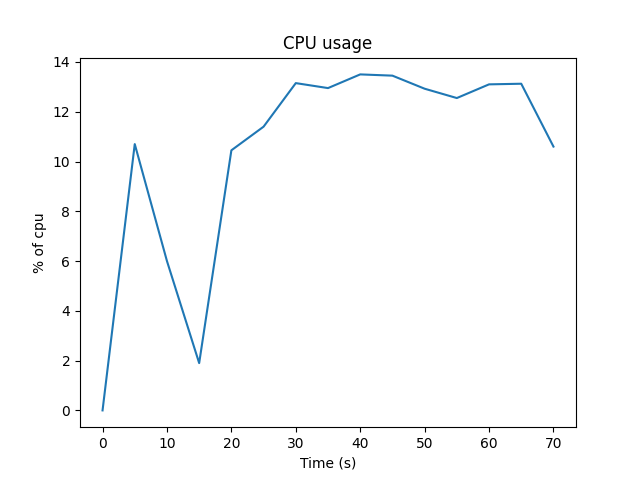
\includegraphics[width=\textwidth]{thesis/images/cpu_operational.png}
        \caption{CPU usage.}
        \label{fig:cpu_usage}
    \end{subfigure}
    \hfill
    \begin{subfigure}[b]{0.45\textwidth}
        \centering
        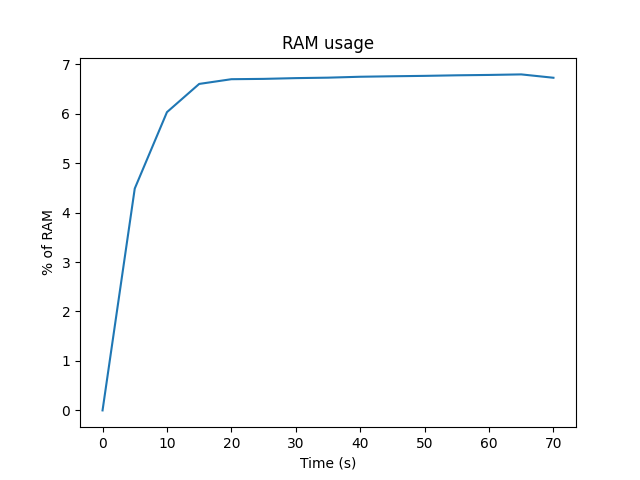
\includegraphics[width=\textwidth]{thesis/images/ram_operational.png}
        \caption{RAM usage.}
        \label{fig:ram_usage}
    \end{subfigure}
    \caption{System resource utilization during the ``operational mode''}
    \label{fig:system_resource_graphs}
\end{figure}

\subsection{Execution time}
As explained in~\ref{sss:automaton_methodology} the execution time between two actions is four seconds, at least. The execution time of the action performed by the robot is not related to the framework. Meanwhile, I performed some tests to find which is the minimal amount of time to wait before receiving the next command and four seconds resulted to be the best choice. But, this amount of time is subjective so, it can be changed by the configuration.

\end{document}
